\section{Introduction}
\label{sec:intro}
In principle, describing an open quantum system is easy: write down a giant wavefunction for the entire universe, place it in an even more gigantic Hilbert space, and evolve it according to the Schrödinger equation.
Somewhere inside that wavefunction lies everything one could wish to know about the system of interest.
In practice, of course, we cannot keep track of every surrounding particle, lattice vibration, stray electromagnetic field, or experimental imperfection and calculate their joint correlated dynamics.
We therefore do what physicists have always done when the universe becomes inconveniently large: draw a boundary.
The degrees of freedom we wish to study are called the \emph{system}; everything beyond this boundary is called the \emph{environment} or \emph{bath}.
Open quantum-system theory asks how the bath affects the system without requiring us to simulate the bath in all its microscopic detail.

The most familiar answers we would see in this regard are those that rely on weak-coupling, short-memory, or related approximations on the baths that lead to time-local master equations.
In the Markovian limit, the system does not need a record of its earlier history in order to determine what happens next.
Markovian master equations provide an extremely successful workhorse for open quantum dynamics, with the Gorini--Kossakowski--Sudarshan--Lindblad form supplying the standard generator of quantum dynamical semigroups~\cite{Gorini1976,Lindblad1976}.
Nevertheless, weak coupling and a clean separation of timescales are not available in every problem.
Structured reservoirs, strong system--bath coupling, slow environmental modes, and delayed feedback can all preserve information about earlier dynamics~\cite{Rivas2014,deVega2017}.
In these regimes, memory is part of the physics rather than a correction that can safely be ignored.

The difficulty is not merely that the environment remembers, but that the system may give us no indication of \emph{what} it remembers if we trace out the bath.
To see this, consider two joint system--environment states at some time $t_1$,
%
\begin{equation}
    \rho_{SE}^{(1)}(t_1) \qquad\text{and}\qquad \rho_{SE}^{(2)}(t_1),
\end{equation}
%
which reduce to exactly the same system state,
%
\begin{equation}
    \operatorname{Tr}_E\!\left[\rho_{SE}^{(1)}(t_1)\right]
    = \operatorname{Tr}_E\!\left[\rho_{SE}^{(2)}(t_1)\right]
    = \rho_S(t_1).
\end{equation}
%
As far as the system density matrix is concerned, these two situations are indistinguishable.
The environment, however, may disagree.
It can retain different states or different correlations with the system in the two cases.
Consequently, evolving both joint states with the same system--environment unitary need not produce the same reduced state at a later time:
%
\begin{equation}
    \operatorname{Tr}_E\!\left[
    U_{2:1}\rho_{SE}^{(1)}(t_1)U_{2:1}^{\dagger} \right] \neq \operatorname{Tr}_E\!\left[
    U_{2:1}\rho_{SE}^{(2)}(t_1)U_{2:1}^{\dagger} \right].
\end{equation}
%
Thus, even perfect knowledge of the present system state need not be sufficient to predict its future.
The information distinguishing the two experiments has simply moved somewhere beyond the boundary we drew earlier.

The limitation becomes sharper when we intervene in our system along the way.
Imagine performing two experiments with different histories and, at an intermediate time $t_1$, discarding the system state and preparing the same fresh state $P$ in both.
This operation---often called a \emph{causal break}---removes any information that could pass directly from the past to the future through the system.
Immediately afterward, both experiments therefore contain the same reduced state,
%
\begin{equation}
    \rho_S^{(1)}(t_1^+)
    = \rho_S^{(2)}(t_1^+)
    = P.
\end{equation}
%
Nevertheless, the intervention acts on a system that may already be correlated with its environment.
A measurement outcome, for example, can condition the environment into a corresponding state, while repreparing $P$ makes the system look identical in every run.
If the later dynamics still depends on the earlier preparation or measurement outcome, then the memory must have travelled across the causal break through the environment.
Such memory can remain hidden in an uninterrupted reduced trajectory, and can even occur when familiar two-time criteria describe the unperturbed evolution as Markovian~\cite{Pollock2018Markov}.

This leaves a state-to-state description with an awkward question.
What map should take $P$ at $t_1$ to the state at $t_2$, if the same $P$ can lead to different futures depending on what happened before it was prepared?
There is no contradiction in quantum mechanics here; rather, we have asked the reduced state to remember information that it no longer contains.
The missing input is the history of interventions---the preparations, controls, and measurements through which the system and its environment arrived at the present experiment.
A complete description of the quantum process must therefore accept an entire ordered sequence of operations, rather than only a density matrix at one particular time.

The process tensor provides precisely such a description~\cite{Pollock2018Framework,Milz2021,Taranto2025}.
For a sequence of interventions $(\mathcal{A}_0,\mathcal{A}_1,\ldots,\mathcal{A}_{n-1})$, it returns the final system state,
%
\begin{equation}
    \rho_S(t_n)
    = \mathcal{T}_{n:0} \bigl[ \mathcal{A}_{n-1},\ldots,\mathcal{A}_0 \bigr],
\end{equation}
%
or, when the interventions contain measurements, the corresponding outcome probabilities and conditional states.
A reduced trajectory tells us what happened under one prescribed history; a process tensor tells us what could have happened had we intervened differently along the way.
It does not reveal every microscopic bath degree of freedom, but retains their complete influence on experiments performed through the system (the mathematical construction behind this statement---including its Choi representation and temporal input and output spaces---will be developed carefully in Sec.~\ref{sec:process-tensors}).
For the present discussion, its operational meaning is enough.
This makes causal breaks, multi-time correlations, instrument sequences, Markov order, and correlations across temporal partitions accessible within one description.
In the Markovian limit, the process separates into independent transformations between successive times; otherwise, its temporal parts remain correlated, recording how information stored in the environment can return later.
Memory thus becomes part of the object being manipulated rather than a feature inferred from a single trajectory.

The generality of a process tensor comes at an exponential cost: every additional intervention time introduces another pair of system indices, thus causing the exponential growth of the representation space of a process tensor, similar to how a many-body wavefunction space grows with the number of particles.
Tensor networks make this manageable by representing the process as a matrix product operator in time, or PT-MPO~\cite{Jorgensen2019}.
The open legs provide the slots for system operations, while the internal bonds carry correlations between different parts of the process.
When these temporal correlations are compressible, singular-value truncations reduce the representation to a controllable bond dimension.
The process tensor is therefore not made small by assumption; it is made useful whenever the environment stores its relevant memory in a compressible temporal space.

\subsection{From microscopic baths to process tensors}
\label{sec:intro-construction}

Having a place to store the memory is only half of the problem.
We still need to work out what the environment writes into it.
For simulations based on a microscopic bath model, constructing a sufficiently accurate and compact PT-MPO is often the main computational task.
Once it is available, changing a preparation, inserting a measurement, or calculating a multi-time correlation amounts to connecting different system operations to its open legs.
For a fixed bath model, coupling, initial bath state, and time grid, the same environmental tensor can therefore support many different experiments without repeating its construction.

Figure~\ref{fig:pt-construction-map} organises several established routes to this object according to the information used to describe the bath: its Gaussian correlations, its individual microscopic modes, or its spatial network.
These are overlapping representations rather than disjoint classes of physical environments.
A collection of harmonic oscillators, for example, may be integrated out analytically, treated mode by mode, or transformed into a chain.
Likewise, a discrete bath need not be non-Gaussian, and a continuous spectrum does not by itself imply Gaussian statistics.
The useful question is which structure we can exploit for what practical purposes.
%
\begin{figure}[htbp]
    \centering
    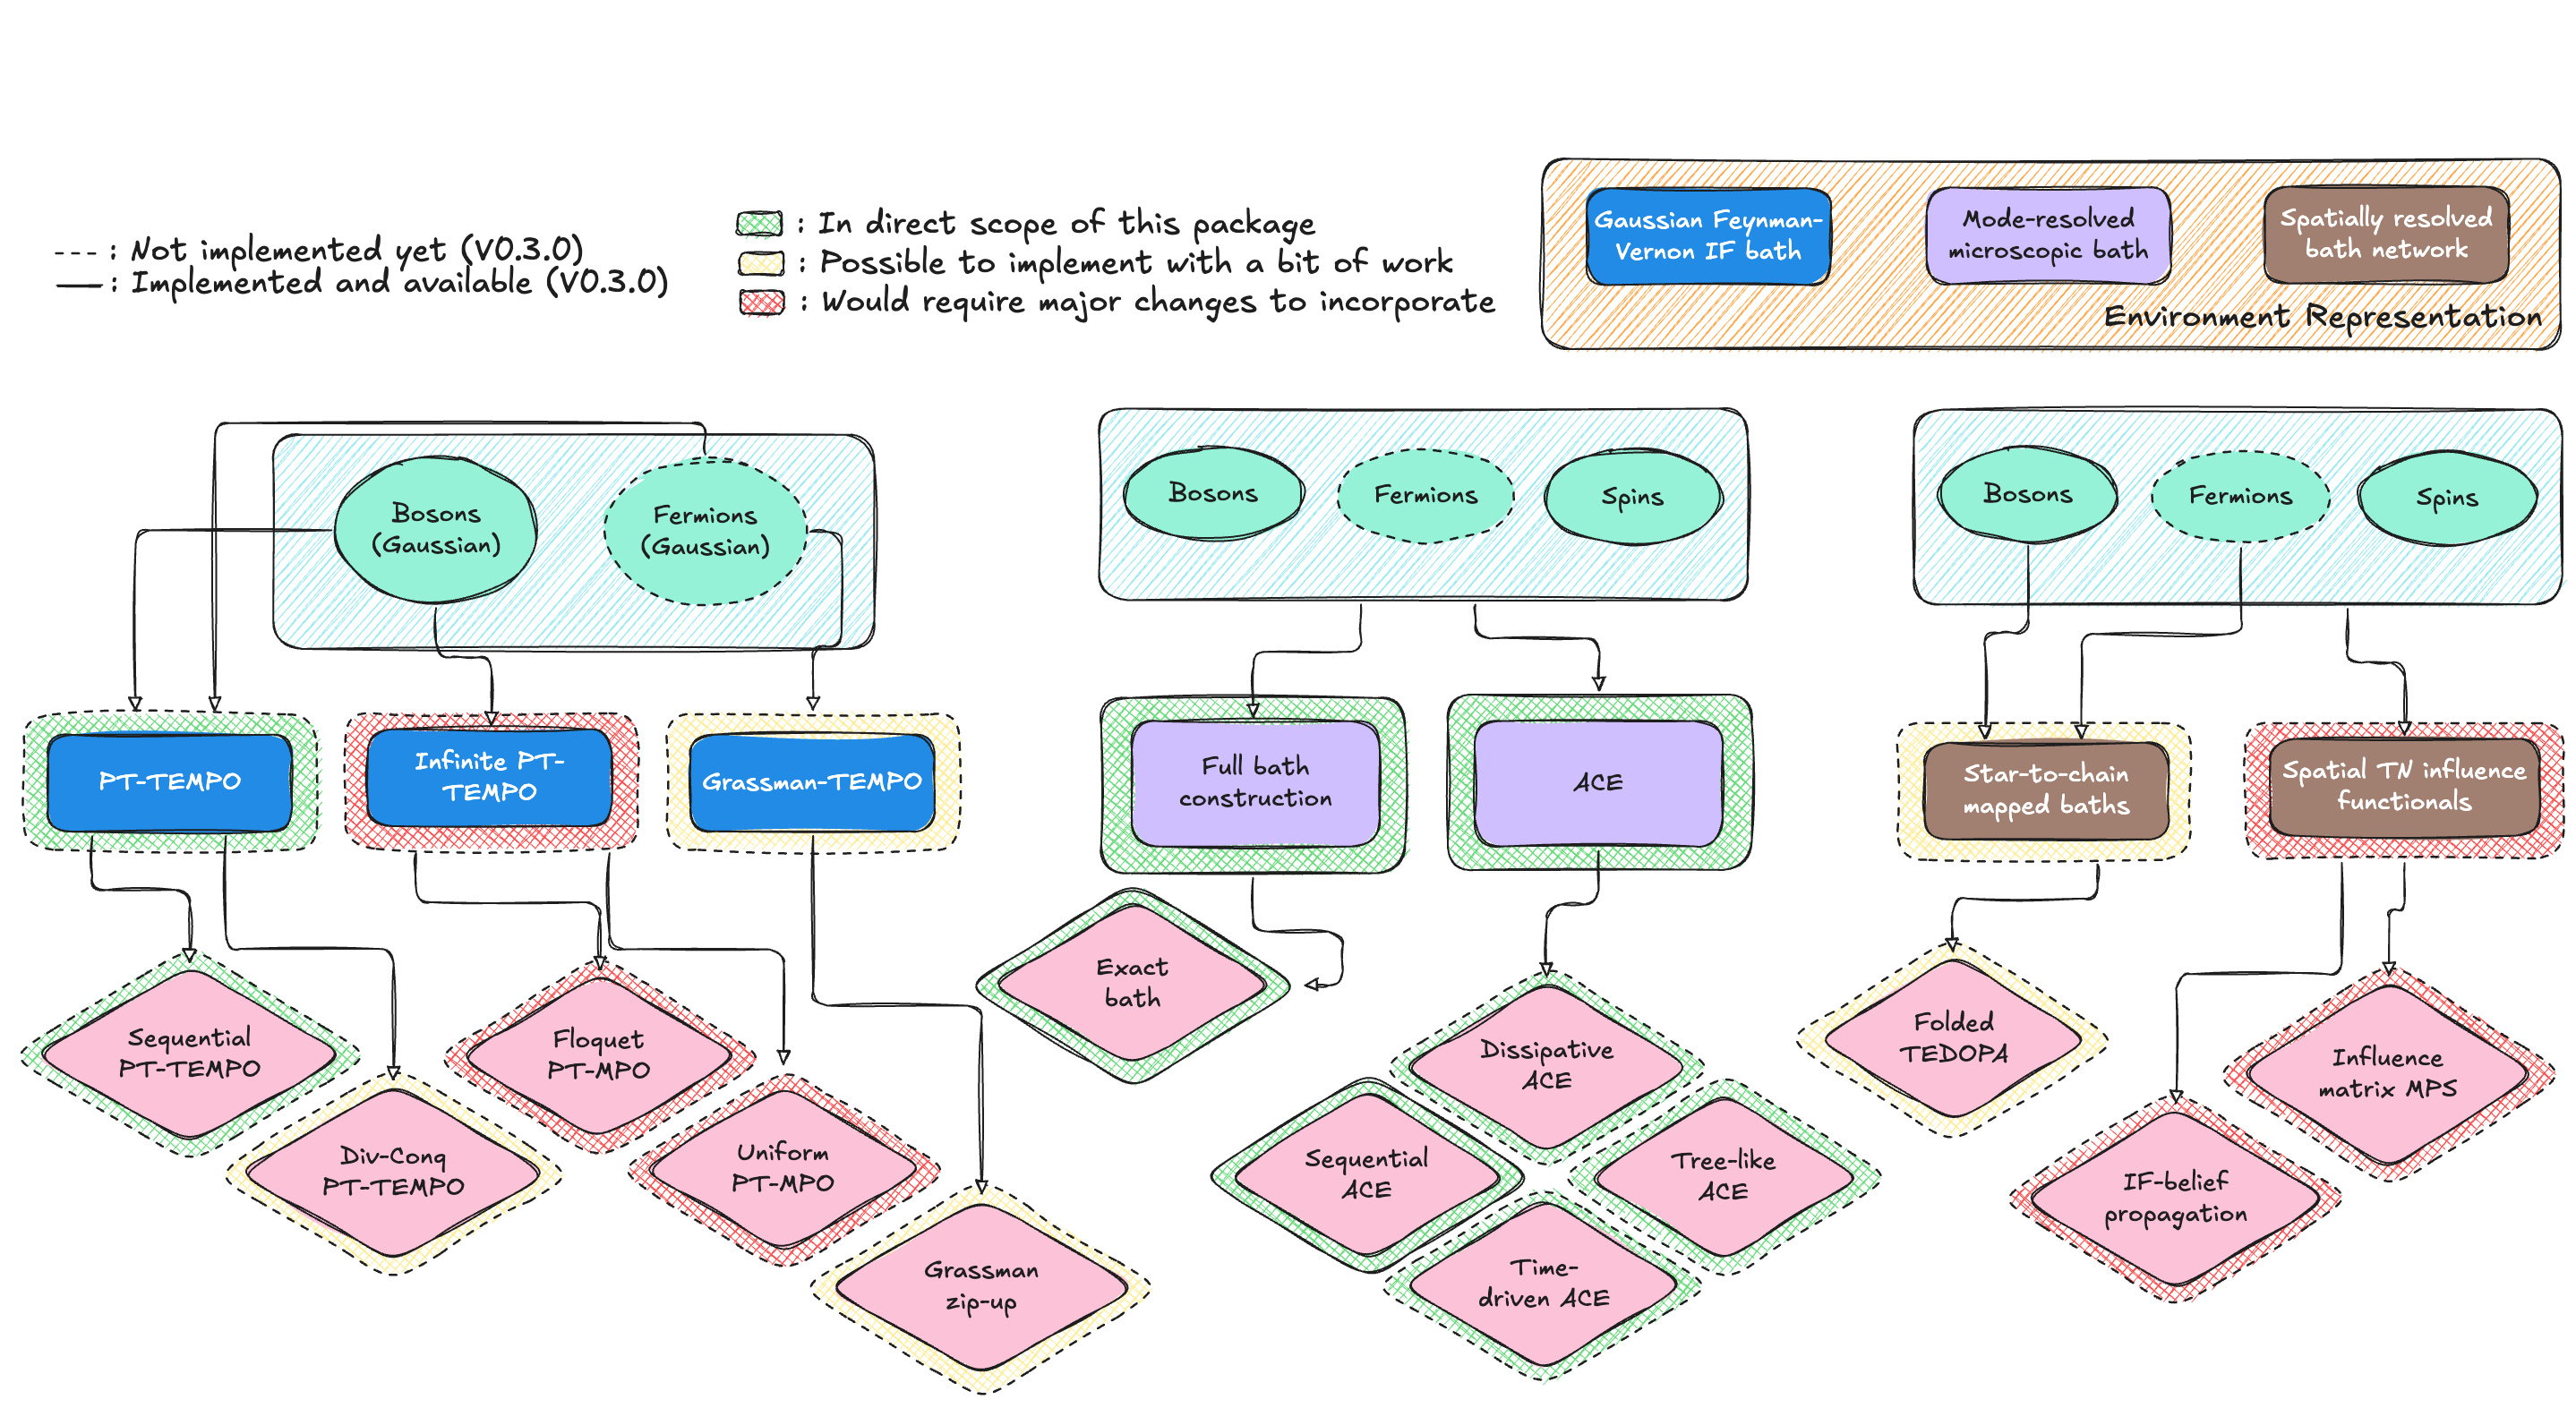
\includegraphics[width=\linewidth]{figures/pt_construction_map.png}
    \caption{Overview of existing tensor-network routes to construc a process tensor.
    The diamonds identify construction and evaluation schemes or specialisations within these families; their roles are described in the text.
    Solid and dashed outlines distinguish whether a method is available in \texttt{ProcessTensors.jl} v0.3.0.
    Green, yellow, and red hatching indicate directions within the package's direct scope, extensions requiring additional development, and approaches requiring major architectural changes, respectively.
    The branches show representative routes.}
    \label{fig:pt-construction-map}
\end{figure}
%

\textbf{\emph{Gaussian influence functionals:}}
The first route removes the bath before compressing its memory.
For a Gaussian environment with the appropriate linear coupling, the Feynman--Vernon influence functional expresses its effect through two-point bath correlations~\cite{FeynmanVernon1963}.
The remaining problem is a sum over system histories, with interactions between different times.
TEMPO represents this temporal structure using tensor networks~\cite{Strathearn2018}; PT-TEMPO reorganises it into a reusable process tensor with the system-operation slots left open~\cite{Jorgensen2019}.
Sequential, divide-and-conquer, and time-translationally invariant finite-time constructions provide different ways of assembling and compressing this network, exploiting repeated temporal structure to reduce the construction effort~\cite{cygorek2024sublinear,guo2024influence}.
For stationary bath correlations, uniTEMPO instead exploits the bath's time translational symmetry and constructs a uniform temporal tensor and boundary vectors, allowing both finite-time evolution and direct access to long-time behaviour through an effective transfer operator~\cite{Link2024Infinite}.
Its direct impact is a much more compressed representation of the process tensor, and its transfer operator can readily be used to obtain steady states. When we wish to drive the system periodically, we can enforce the same time translation symmetry with a modulo of the time period of driving, and obtain Floquet dynamics using the same machinery~\cite{Mickiewicz2026Floquet}.
Fermionic Gaussian reservoirs require their anticommutation structure to be retained: Grassmann TEMPO supplies a corresponding influence-functional construction, while its zip-up scheme evaluates observables without first forming one large combined temporal tensor~\cite{Chen2024GTEMPO}.
Infinite Grassmann constructions additionally give direct access to steady-state impurity correlations and transport without explicitly following the full transient~\cite{GuoChen2024InfiniteSteady}.
Related fermionic influence-functional MPS constructions also address nonequilibrium impurity models~\cite{Thoenniss2023Impurity,Ng2023Impurity}.
These approaches are particularly useful for structured thermal reservoirs and impurity problems, since the bath can be specified through correlations or spectral data without explicitly retaining every mode.
Their efficiency nevertheless depends on temporal compressibility; long memory, strong coupling, and additional coupling channels can make the bonds expensive.
Moreover, the Gaussian reduction is a physical restriction, whereas stationarity is an additional restriction of particular acceleration schemes rather than of finite-time influence functionals themselves.

\textbf{\emph{Mode-resolved microscopic environments:}}
The second route starts with the bath degrees of freedom themselves.
For a small environment, we can construct the joint propagators directly and trace out the bath while retaining the system's temporal input and output legs (``Exact bath'' diamond in Fig.~\ref{fig:pt-construction-map}).
This provides a useful reference construction, although its uncompressed memory space grows with the full bath Liouville space.
Automated compression of environments (ACE) makes a more scalable construction possible when the environment consists of independent modes, initially in a product state~\cite{Cygorek2022}.
Each mode contributes a small process tensor, and their combined influence is compressed as the modes are incorporated.
The modes need not be harmonic or Gaussian: spins, truncated oscillators, and more general finite-dimensional constituents can be treated through their microscopic propagators.
Sequential ACE adds these contributions one at a time; tree-like ACE merges them hierarchically and uses additional compression sweeps to improve the construction~\cite{Cygorek2024Treelike}.
Time-dependent mode propagators and local dissipative generators extend the same microscopic viewpoint to driven or damped modes~\cite{Cygorek2022,CygorekGauger2024}.
The corresponding diamonds in the figure describe extensions of the local dynamics as well as choices of contraction order.
This flexibility is attractive when individual environmental constituents matter or Gaussian assumptions fail.
It does not make a large continuum bath inexpensive by default: the mode discretisation, local Hilbert-space cutoffs, time steps, and compression must all be converged.
Intermode interactions and initially correlated modes also lie beyond the standard independent-mode construction unless they are incorporated into larger jointly treated units.
For a Gaussian continuum, using its analytically known influence functional can therefore avoid work that the more general microscopic route must perform explicitly.

\textbf{\emph{Spatially resolved bath networks:}}
The third route retains how environmental degrees of freedom connect to one another.
For linearly coupled free bosonic or fermionic reservoirs, star-to-chain mappings transform the bath into a nearest-neighbour chain; orthogonal-polynomial mappings and TEDOPA established this route to explicit-environment tensor-network simulations~\cite{Chin2010,Prior2010}.
Mapping and evolving the chain alone does not produce a process tensor.
To obtain one, the forward and backward evolution networks can be folded together and contracted over the bath while the intervention legs remain open, leaving a tensor network along time~\cite{ye2021influence,cerezo2025spatiotemporal}.
This is the construction route labelled ``folded TEDOPA'' in the figure.
Alternatively, the environment may already be an interacting lattice, with a local subsystem playing the role of the open system.
Influence-matrix MPS methods contract the surrounding space-time network in the spatial direction, or solve a spatial self-consistency problem, to encode its effect on the subsystem's histories~\cite{Lerose2021Influence,ye2021influence}.
Influence-functional belief propagation extends this viewpoint to branching networks by passing temporal influence tensors between neighbouring sites~\cite{Park2025Belief}.
Boundary influence tensors become a system process tensor only after the appropriate local tensors are attached and the intervention slots retained.
These methods give access to interacting, non-Gaussian environments and connect open-system questions to many-body dynamics.
Their practical reach is limited by spatial and temporal entanglement, bath-size and local-basis truncations where applicable, and, for loopy networks, the quality of the spatial approximation.

%%%%%%%%%%%%%%%%%%%%%%%%%%%%%%%%%%%%%%%%%%%%%%%%%%%%%%%%%%%%%%%%%%%%%%%%%%%
\subsection{Software and the scope of this package}
\label{sec:intro-software}

Several open-source packages already turn these constructions into useful numerical tools.
\texttt{OQuPy} implements PT-TEMPO for Gaussian bosonic environments and uses the resulting process tensors for dynamics, multi-time correlations, and control, including extensions to coupled systems~\cite{Fux2024}.
The C++ \texttt{ACE} toolkit provides the independent-mode ACE construction alongside Gaussian-bath PT-MPO algorithms, including divide-and-conquer schemes, with facilities for saving, reusing, and combining environmental tensors~\cite{CygorekGauger2024}.
\texttt{UniformTEMPO.jl} supplies the uniform construction for infinite process tensors~\cite{Link2024Infinite,UniformTEMPOSoftware}, while \texttt{GTEMPO.jl} implements Grassmann influence-functional methods for fermionic impurity problems~\cite{Chen2024GTEMPO,XuGuoChen2024GTEMPO,GTEMPOSoftware}.
Within Julia, \texttt{QuantumDynamics.jl} offers a broader collection of influence-functional, tensor-network, and other open-system methods~\cite{Bose2023}, and \texttt{MPSDynamics.jl} provides explicit-environment simulations based on thermalised TEDOPA although it not yet directly uses PT-MPO construction~\cite{Lacroix2024}.
Research codes such as \texttt{imcode} provide complementary influence-matrix calculations for lattice and impurity settings~\cite{IMCodeSoftware}.
Related path-integral tools, such as \texttt{PathSum}, also form part of this wider numerical landscape~\cite{Kundu2023PathSum}.
For broader comparisons, including methods outside direct PT-MPO construction, we refer readers to the PRX perspective by Keeling, Stoudenmire, Ba\~nuls, and Reichman~\cite{Keeling2026} and the review by Lacroix and collaborators~\cite{LacroixReview2026}.

\texttt{ProcessTensors.jl} brings a particular emphasis to this landscape: constructing finite-time process tensors and making their operational content accessible in an intuitive Julia language.
We use \texttt{ITensors.jl} and \texttt{ITensorMPS.jl} as the tensor-network foundation~\cite{Fishman2022}.
Named indices and tags let the code follow the same question as a tensor diagram: which legs describe the system, which carry memory, and which should be connected to an intervention?
The Liouville-space interface then provides a common language for process tensors, system operations, and their contractions.
The present release centres on direct finite-bath construction and sequential ACE, providing both a small-system reference and a compressed route to more general independent-mode environments.
With the process available, users can explore preparations, instrument sequences, conditional statistics, and temporal correlations through the same representation.
The contribution is this connection between construction, operational use, and an accessible implementation, building on the established algorithms described above.

The figure also places the present implementation within a development roadmap.
We describe how alternative constructors can target the same finite-time PT-MPO interface, so that improvements in bath construction can be reused by the existing evaluation routines.
Nearer extensions include time-dependent and dissipative mode propagators, tree-like ACE, and Gaussian PT-TEMPO construction; divide-and-conquer schemes and chain-based constructions require additional algorithmic machinery.
Fermionic support must also account consistently for parity and operator ordering.
Uniform and Floquet process tensors, and spatial influence-functional networks, require more substantial changes to the representation or construction infrastructure.
We provide the details of these extensions in the following sections.

The remainder of this paper develops this connection between theory and use step by step.
We introduce the Liouville-space and tensor-network conventions, construct process tensors and their compressed representations, and explain how system operations and instruments extract experimentally meaningful quantities from them.
Worked examples connect these ingredients to numerical workflows, followed by benchmarks and the development roadmap.
Throughout, equations, tensor diagrams, and Julia code are presented together so that the same operation can be followed in each language.
The theory and Julia markers in the table of contents indicate the predominant emphasis of each section and help readers choose a route through the material.
Students can follow the construction from its physical meaning to a working calculation, while experienced readers can move directly to the implementation details, examples, and extension points relevant to their own problems.
